\section{ATLAS Detector Upgrade}

The Large Hadron Collider (LHC), run by CERN at the Franco-Swiss border near Geneva, is a circular accelerator with 27 km of acceleration pipes, is the largest scientific instrument ever designed and built for scientific research. Successfully commissioned in March 2010 for proton-proton collision with a 7 GeV centre-of-mass energy.\\
The LHC is pusshing the limits of human knowledge, enabling physicist to go beyond Standar Model (SM): the enigmatic Higgs boson, mysterious Dark Matter and the world of supersymetry are just three of the long-awaited mysterous that the LHC will unveil. The announcement given by CERN on 4 July 2012 about the discovery of new boson at 125-126 GeV, almost certainly the long awaited Higgs particle, is the first fundamental discovery, hopefully the first of a series, that the LHC can deliver.\\
Such discovery was thanks to the different multipurpose detectors located at the four interaction points (IP); ALICE, LHCb, CMS and ATLAS. This last one is the detector where our university is taking part.\\
A mutipurpose detector designed to explore proton-proton colissions at center of mass up to $\sqrt{s}=14GeV$. Such energy has been achived from 2015 and successfuly working with a luminosity of $1x10^{34}cm^{-2}s^{-1}$ from 2016.\\
\begin{figure}[h]
		\centering
		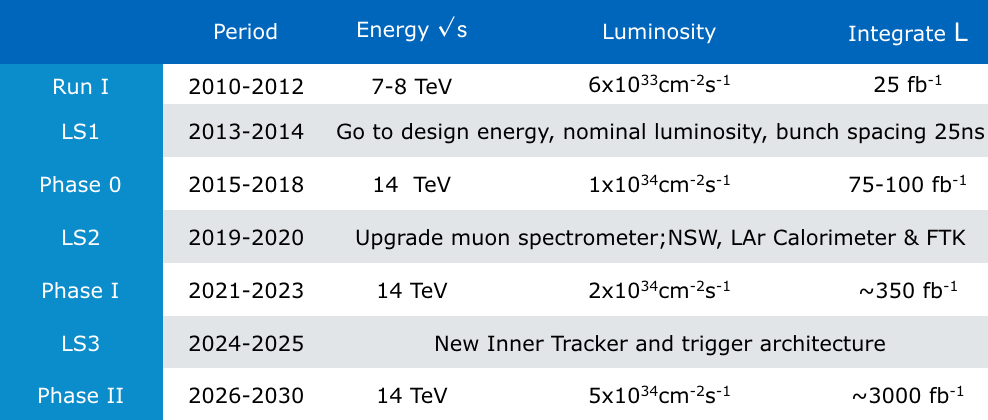
\includegraphics[width=0.8\textwidth]{LHC_program_table.png}
		\caption{LCH Schedule}\label{fig:a}
\end{figure}
In manner to fullfill the LHC program (in fig.\ref{fig:a}), and in order to benefit from the expected high luminosity performance that will be provided by the Phase-I upgraded LHC, the first station of ATLAS muon end-cap system (Small Wheel, SW) will need to be replaced. The New Small Wheel (NSW) will have to operate in a high background radiation region (upto 15kHz/cm$^2$) while reconstructing muon tracks with high precision as well as furnishing information for the Level-1 trigger. These performance criteria are demanding. In particular, the precision reconstruction of tracks for offline analysis requires a spatial resolution about 100 $\mu$m, and the Level-1 trigger track segments have to be reconstructed online with an angular resolution of approximately 1mrad. The NSW will have to chamber technologies, one primarily devoted to the Level-1 trigger function (small-strip Thin Gap Chambers, sTGC) and one dedicated to precision tracking (Micromegas detectors, MM). The sTGC are primarily deployed for triggering given their single bunch corssing identification capability. The MM detectors have exceptional precision tracking capabilities due to their small gap (5mm) and strip pitch (approximately 0.5mm). Such a precision is crucial to maintain the current ATLAS muon momentum resolution in the high background environment of the upgraded LHC. The MM chambers can, at the same time, confirm the existence of a track segments found by the muon end-cap middle station (Big Wheels) online. The sTGC also has the ability to measure offline muon tracks with good precision, so the sTGC-MM chamber technology combination forms a fully redundant detector system for triggering and tracking both for online and offline functions. This detector combination has been designed to be ablo to also provide excellente performance for the eventual High Luminosity LHC upgrade. 



\section{Small-strip Thing Gap Chamber}
According to literature it's posible to define a Thin Gap Chamber (TGC) as a multiwire proporptional chamber.\par

\section{Construction process}

\section{Gain and uniformity}

\section{Working under high $\gamma$ rate}

\section{Spatial resolution strips}

\section{Charge sharing between pads}

\section{summary}
